\documentclass[UTF8]{ctexart}
\usepackage{amsmath}
\usepackage{float}
\usepackage{cases} 
\usepackage{cite}
\usepackage{graphicx}
\usepackage[margin=1in]{geometry}
\geometry{a4paper}
\usepackage{fancyhdr}
\usepackage{booktabs}
\pagestyle{fancy}
\usepackage[version=4]{mhchem}
\fancyhf{}

\title{底物浓度对酶促反应速度的影响——米氏常数的测定}
\author{522111910161 尚子翔}
\date{\today}
\pagenumbering{arabic}

\begin{document}
	
	\fancyhead[L]{}
	\fancyhead[C]{底物浓度对酶促反应速度的影响——米氏常数的测定}
	\fancyfoot[C]{\thepage}
	
	\maketitle
	\tableofcontents
	\newpage
	
	\section{实验目的}
	\begin{enumerate}
		\item 了解底物浓度对酶促反应速度的影响
		\item 了解米氏常数Km的数学意义和生物学意义
		\item 通过甲醛滴定法测定胰蛋白酶在不同底物浓度下经不同时间的反应进度
		\item 采用双倒数作图法测定胰蛋白酶的米氏常数
	\end{enumerate}
	
	\section{实验原理}
	\subsection{酶促反应}
	酶是由生命体产生的催化剂,具有针对特定底物的高度选择性和催化效率,可在温和条件下促进生物体内化学反应的进行。酶催化反应是指由酶作为催化剂促进的化学反应,其高效率和特异性使其仅催化热力学允许的反应,并不影响反应的平衡状态。其作用机制在于降低反应的活化能。酶催反应受到多种因素的影响,包括温度、酸碱度、酶浓度、底物浓度、抑制剂、激活剂以及反应产物。温度的升高可加快反应速率,但也可能导致酶的失活。因此,存在最适温度,使反应速率最大化。酶活性受pH影响,过高或过低的pH值可能改变酶的构象并导致酶失活。因此存在最适pH,有利于酶、底物和辅因子的结合和解离,从而使酶催反应速度达到最大值。
	
	胰蛋白酶是一种蛋白酶,从牛、羊、猪的胰脏提取,属于丝氨酸蛋白水解酶,作为消化酶发挥作用。胰蛋白酶具有严格的特异性,专门针对由碱性氨基酸精氨酸和亮氨酸组成的肽键。该酶易溶于水,不溶于三氯甲烷、乙醇、乙醚和甘油。其最适pH范围为8.0至9.0,且在pH为1.8时,经短时煮沸几乎不失活。此外,$Ca^{2+}$对胰蛋白酶具有保护和激活作用。
		
		本研究在中性pH条件下,以37℃为反应温度,研究了胰蛋白酶对酪蛋白水解的反应速率。
	\subsection{酶促反应速度与底物浓度的关系}
	对于单底物酶促反应反应S→P,在其他条件均为最适,仅底物浓度不同的条件下,通过一定时间内产物变化率计算反应速率:\[V=\frac{\Delta [P]}{\Delta t}\]
		
	研究发现,在底物浓度很低时,酶促反应是一级反应;当底物浓度处于中间范围时,酶促反应是混合级反应;当底物浓度继续增加时,酶催化能力趋近饱和,酶促反应向零级反应过渡,即反应不受底物浓度的影响,而只与酶活性浓度成正比;最终酶催化能力完全饱和,达到最大反应速率。
	
	\subsection{甲醛滴定法}
水溶液中的氨基酸为兼性离子,因而不能直接用碱滴定氨基酸的羧基。甲醛可与氨基酸上的 \(NH_3^+\) 结合,形成 \(NH-CH_2OH\)、\(N(CH_2-OH)_2\) 等羟甲基衍生物,使 \(NH_3^+\) 上的 \(H^+\) 游离出来,这样就可以用碱滴定 \(NH_3^+\) 解离的 \(H^+\),计算氨基酸的含量。

同时,甲醛具有较高的反应活性,可以和带有 \(OH\)(羟基)、 \(SH\)(巯基)、 \(NH_2\)(氨基)基团的分子发生亲核加成反应,使胰蛋白酶变性失活,使酶促反应立即终止。此时溶液中不再有新的氨基酸产生,测得的产物含量即为加入甲醛时溶液中的产物含量。
	\subsection{米氏常数$K_m$与米氏方程的推导}
	首先,大量过量的底物(S)可逆地与酶结合(E)以形成酶-底物复合物(ES):
	\begin{center}
		\ce{E + S <=>T[$k_1$][$k_{-1}$] ES}
	\end{center}
	
	基质中的复合物又转化为产物(P):
	\begin{center}
		\ce{ES ->T[$k_2$] E + P}
	\end{center}
	
	由于该机制中的第二步是缓慢的,反应的速率定律由下式给出:
	
	\[V = k_2[ES]\]
	
	这个速率定律的缺点是它包含了一种中间体的浓度[ES]。由于中间体的浓度通常难以测量,因此需要从速率定律中消除它。为此,Michaelis-Menten将稳态假说近似应用于ES浓度;换言之,假设ES浓度在大部分反应期间是合理恒定的。因此其产生和分解的速率应当相等,即:
	
	\[k_1[E][S]=(k_{-1}+k_2)[ES]\]
	
	从而有:
	
	\[\frac{[S][E]}{[ES]} = \frac{k_{-1} + k_2}{k_1}\]
	
	定义米氏常数$K_m$:
	
	\[K_m=\frac{k_{-1} + k_2}{k_1}\]
	
	游离酶浓度[E]难以测得,而总酶浓度[E]T容易测得,根据:
	
	\[[E]_T = [E] + [ES]\]
	
	得到:
	
	\[V=k_2[E]_T \frac{[S]}{[S]+K_m}\]
	
	当$[S] >> K_m$ :
	
	\[V_m=k_2[E]_T\]
	
	$V_m$表示反映的最大速率。于是我们得到了米氏方程(Michaelis-Menten equation):
	
	\[V=V_M \frac{S}{[S]+K_m}\]
	\subsection{双倒数作图法}
	对于米氏方程两边同时取倒数,将其变形为:
	\[\frac{1}{V} = \frac{K_m}{V_m} \times \frac{1}{[S]} + \frac{1}{V_m}\]
	
	以反应速率倒数对底物浓度倒数作图,图像如下:
	
	\begin{figure}[H]
		\centering
		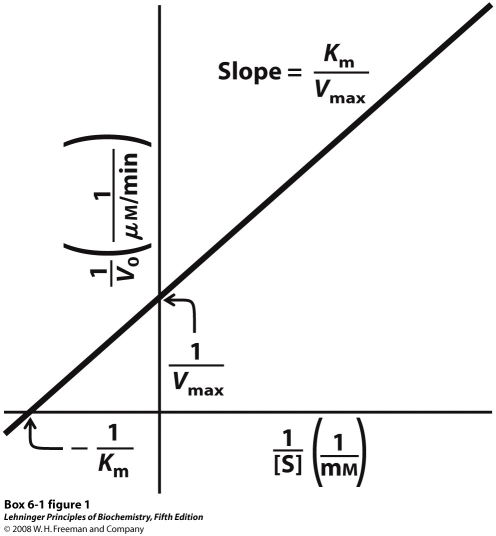
\includegraphics[width=0.5\textwidth]{1.png}
		\caption{双倒数作图法}
		\label{fig:example}
	\end{figure}
	\section{实验操作与流程}
	\subsection{实验试剂与仪器}
	\begin{itemize}
		\item 实验试剂:胰蛋白酶粉、40g/L 酪蛋白溶液、甲醛、0.1mol/L 氢氧化钠溶液、0.25\% 酚酞试剂、去离子水
		\item 实验仪器:恒温水浴锅、碱式滴定管、秒表、量筒、10mL移液管、5mL移液管、洗耳球、微量移液器及枪头、烧杯、锥形瓶、50mL容量瓶、胶头滴管
	\end{itemize}
	\subsection{实验步骤}
	\subsubsection{制备酪蛋白溶液和胰蛋白酶溶液}
	量取1g 胰蛋白酶粉于烧杯,加入25ml 去离子水溶解,放入37℃恒温水浴锅保温。
	
	使用40g/L 酪蛋白母液按下表配制四组不同浓度的酪蛋白溶液,放入37℃恒温水浴锅保温。
	
	\begin{table}[h]
		\centering
		\caption{酪蛋白溶液的配置}
		\begin{tabular}{ccc}
			\toprule
			配制的酪蛋白溶液浓度 g/L & 加入酪蛋白母液体积 mL & 加入去离子水体积 mL \\
			\midrule
			40 & 50 & 0 \\
			30 & 37.5 & 12.5 \\
			20 & 25 & 25 \\
			10 & 12.5 & 37.5 \\
			\bottomrule
		\end{tabular}
	\end{table}
	\subsubsection{制备中性甲醛溶液}
	量取75mL 甲醛于锥形瓶,加入15mL 0.25\% 酚酞试剂,及时用铝箔纸封口。用0.1mol/L 氢氧化钠溶液将其滴定至刚好呈微红色,即制得中性甲醛溶液,及时用铝箔纸封口。
	
	分别量取5mL 中性甲醛溶液加入四个50mL锥形瓶,加入后用铝箔纸封口。
	\subsubsection{反应}
	将酪蛋白溶液倒入100mL锥形瓶,用移液管量取5mL 胰蛋白酶溶液,加入锥形瓶的同时开始计时,并振荡混匀。
	
	在20s、2min、4min、6min分别用移液管移取10mL 反应物,分别加入四个装有中性甲醛溶液的锥形瓶,加入的同时按下秒表计次,将50mL锥形瓶振荡混匀,及时用铝箔纸封口。
	
	\subsubsection{甲醛滴定法测定反应进度}
	用0.1mol/L 氢氧化钠溶液滴定50mL锥形瓶中混合液,滴定至混合液恰好呈微红色时停止滴定,记录滴定前后滴定管读书,计算并记录所用氢氧化钠体积。滴定后的废液及时倒入指定废液桶。
	\subsection{注意事项}
	\begin{itemize}
		\item 甲醛易挥发且有毒性,应注意实验室通风,在通风橱内量取甲醛,对于含甲醛的容器不用时要及时用铝箔纸封口,含甲醛的废液应及时倒入指定废液桶。
		\item 水浴保温酪蛋白溶液和胰蛋白酶溶液时应注意编号和放止容器倾倒,从水浴锅拿出试剂后应及时开始反应。
		\item 加入酪蛋白溶液和胰蛋白酶溶液前应将其振荡混匀(胰蛋白酶溶液易产生沉淀)。
		\item 反应中应不时振荡混匀反应液。
		\item 滴定时氢氧化钠溶液用量较少(4mL以内),应避免滴定过量。
	\end{itemize}
	\section{实验结果记录}
	称得胰蛋白酶:1.000g  \ 酪蛋白母液:40g/L \  滴定用NaOH溶液浓度:0.100mol/L
        \begin{table}[H]
        \centering
        \begin{tabular}{cccccccc}
        \toprule
        \multicolumn{2}{c}{10g/L} & \multicolumn{2}{c}{20g/L} & \multicolumn{2}{c}{30g/L} & \multicolumn{2}{c}{40g/L} \\
        \cmidrule(r){1-2} \cmidrule(lr){3-4} \cmidrule(lr){5-6} \cmidrule(l){7-8}
        t/min & V/ml & t/min & V/ml & t/min & V/ml & t/min & V/ml \\
        \midrule
        0.5 & 0.98 & 0.57 & 1.74 & 0.45 & 2.10 & 0.40 & 2.50 \\
        1.25 & 1.14 & 1.12 & 1.86 & 1.07 & 2.38 & 1.05 & 3.50 \\
        3.15 & 1.22 & 3.05 & 2.30 & 3.05 & 2.92 & 3.02 & 3.82 \\
        5.08 & 1.76 & 5.05 & 2.54 & 5.00 & 3.22 & 4.98 & 3.98 \\
        \bottomrule
        \end{tabular}
        \caption{实验记录}
        \end{table}
		
	\section{实验结果分析与讨论}
        \subsection{数据处理}
        首先,做出$V_{NaOH} - T$图像,通过线性拟合,斜率即为四个不同浓度下反应的速度,单位是mol/s。
        \begin{figure}[H]
             \centering
             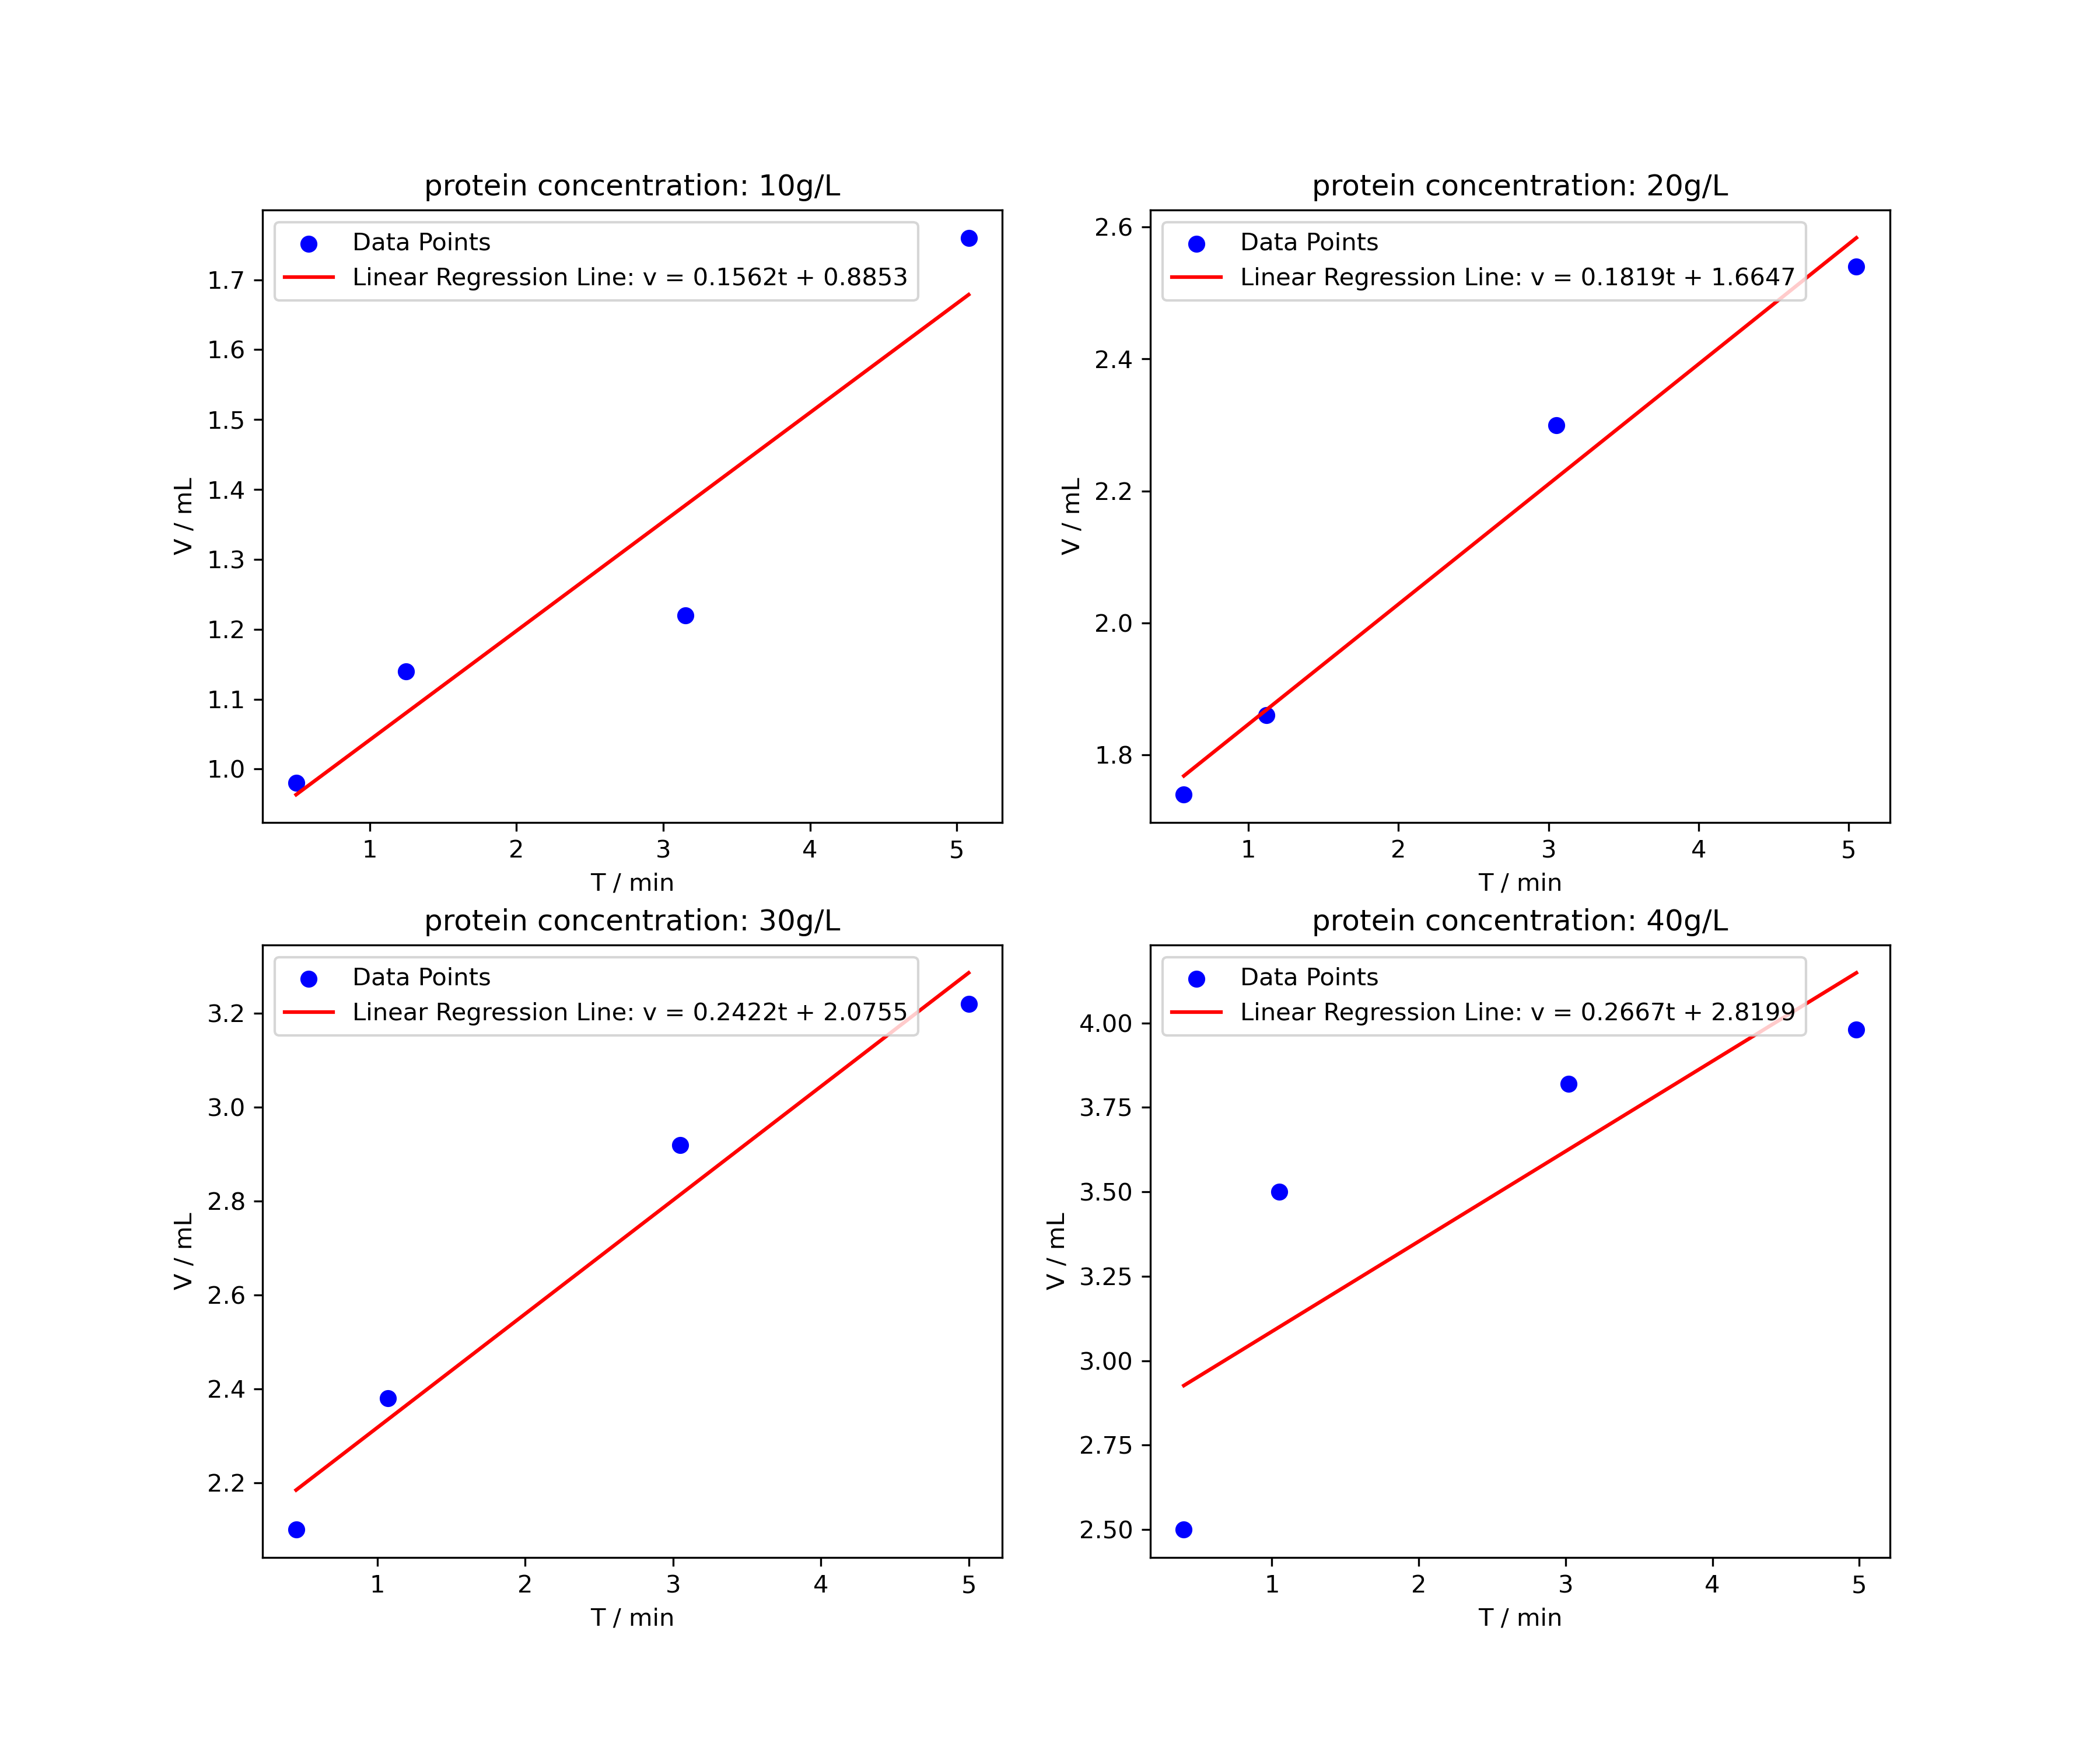
\includegraphics[width=1\linewidth]{out1.png}
             \caption{$V_{NaOH} - T$线性拟合结果与图像}
             \label{fig:enter-label}
         \end{figure}
    \newpage
        再根据已经得到的反应速率以及对应的浓度,通过双倒数作图法,作出$\frac{1}{V} \sim \frac{1}{[S]}$图,得出米氏常数和最大反应速率。
        \begin{figure}[H]
            \centering
            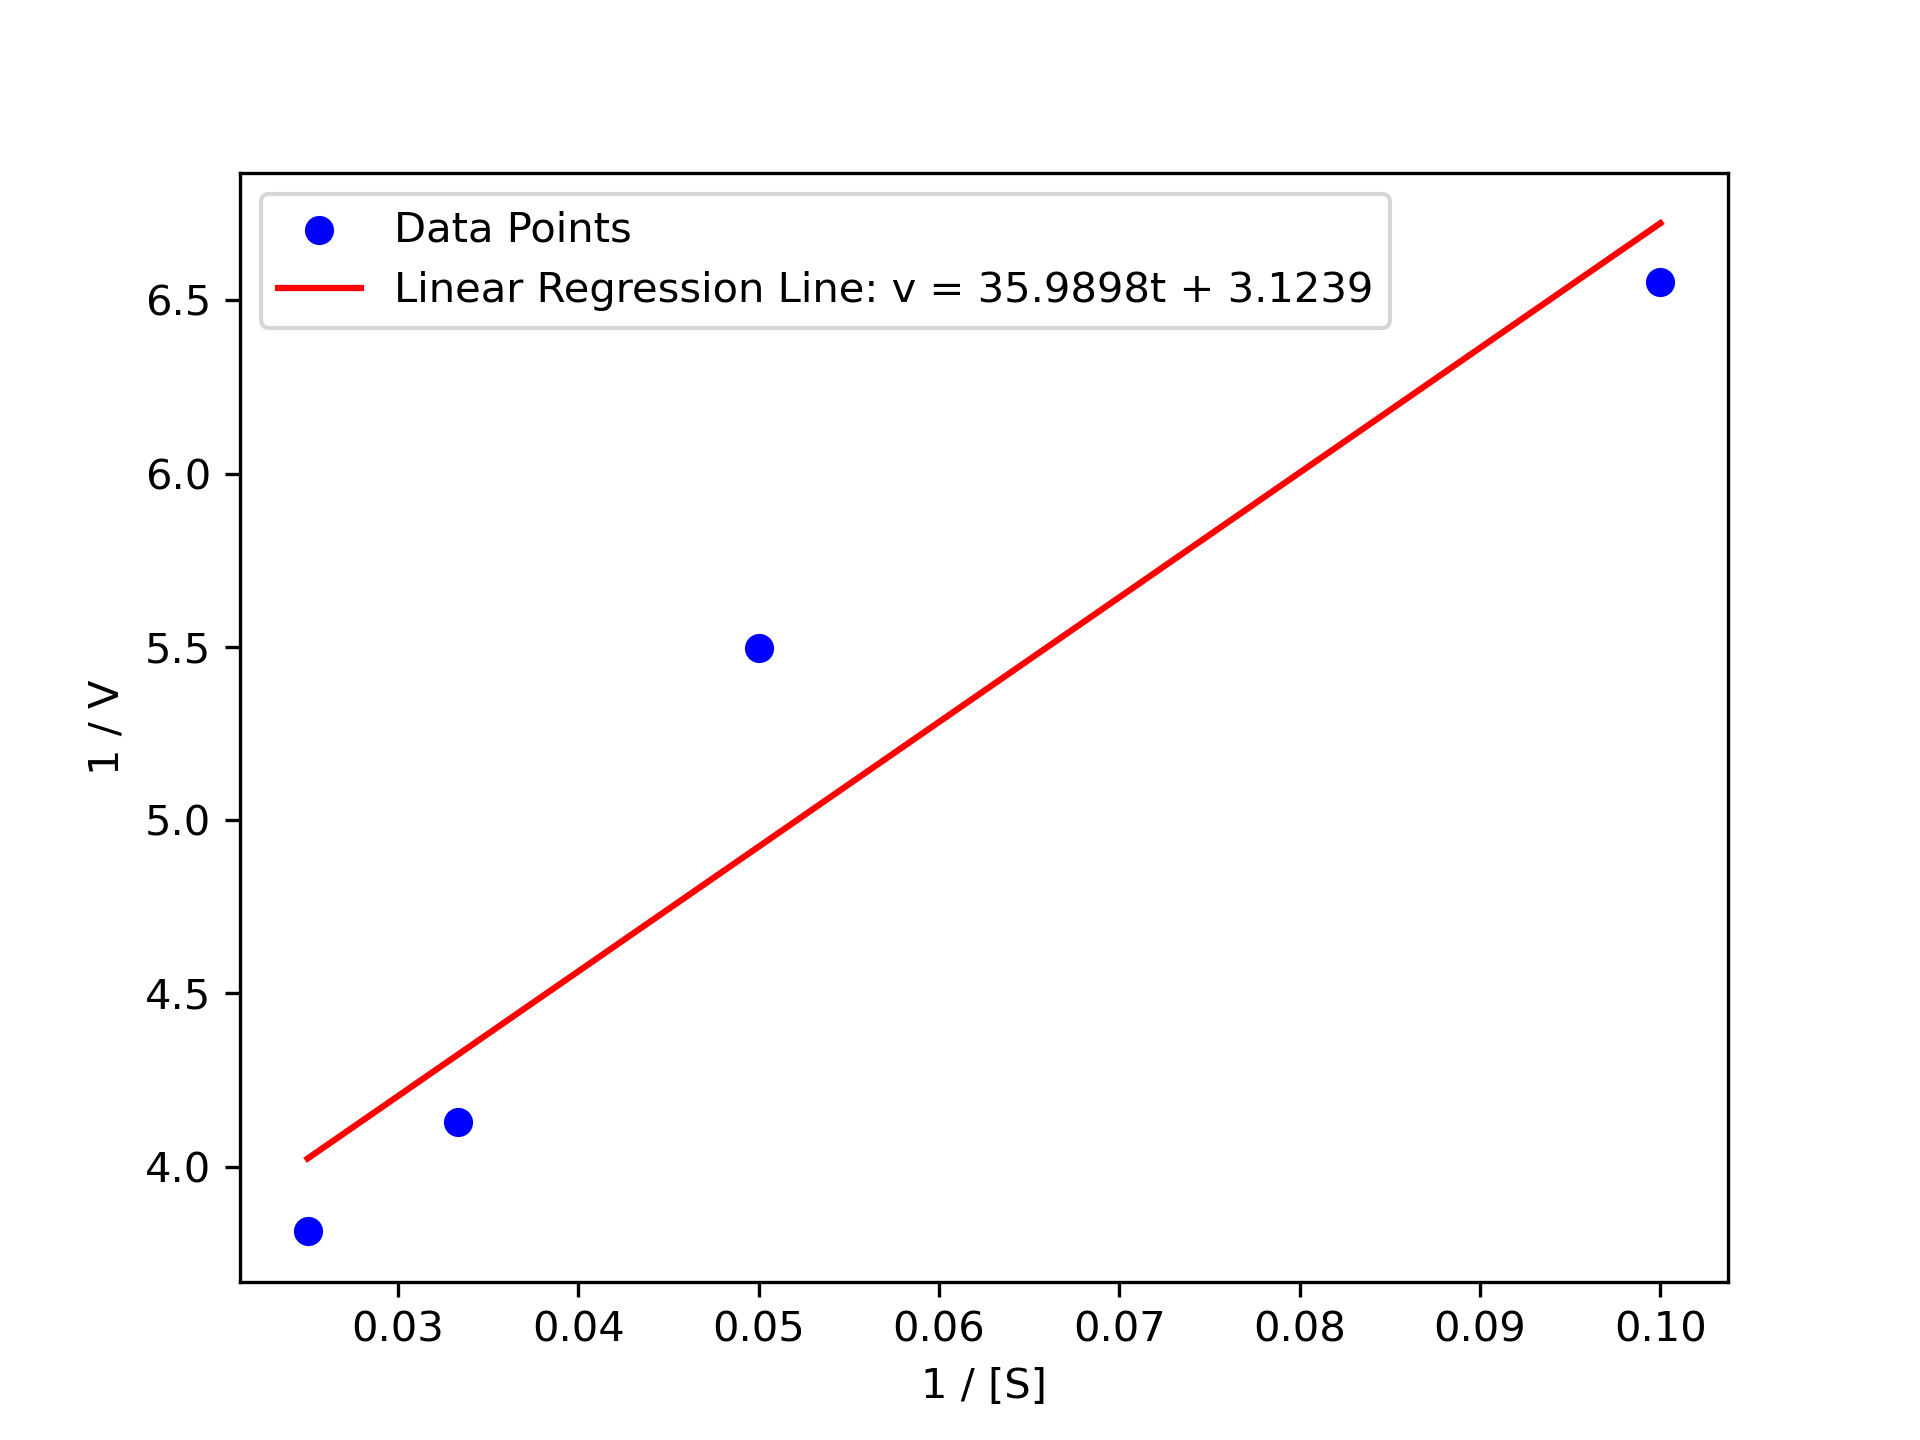
\includegraphics[width=0.5\linewidth]{out2.png}
            \caption{$\frac{1}{V} \sim \frac{1}{[S]}$线性拟合结果与图像}
            \label{fig:enter-label}
        \end{figure}
        根据斜率$k = \frac{K_m}{V_{max}} = 35.9898$,截距$b = \frac{1}{V_{max}} = 3.1239$, 可以得出:
        \[V_{max} = 0.3201mol/s\]
        \[K_m = 11.5208g/L\]
        \subsection{分析与讨论}
        $\frac{1}{V} \sim \frac{1}{[S]}$图拟合结果的pearson相关系数为0.95327,从图上看第二组实验误差比较大,降低了两者的相关性。在20g/L中测得的速率偏小,我推测误差来源可能是:
        \begin{enumerate}
            \item 将胰蛋白酶加入酪蛋白溶液后并没有充分搅拌,从而反应速率相较其他组比较小。
            \item 胰蛋白酶在第一组实验后没有及时放回水浴锅,温度比较低,酶的活性降低,反应速率偏低。
        \end{enumerate}

        测40g/L酪蛋白溶液中的反应速率数据在图中表现出误差较大,我猜测导致4组数据误差均比较大的原因是:烧杯或者容量瓶没有完全清洗干净,上一组残留的溶液导致滴定非常不准确。

        其他可能导致误差的原因还有:
        \begin{enumerate}
            \item NaOH滴定时不够仔细,滴定结束后溶液颜色不同。
            \item 秒表开始计时与结束计时的时刻存在误差。
            \item 准备的酪蛋白母液不足,新旧母液浓度可能存在差异。
        \end{enumerate}
        \subsection{总结与改进}
        \subsubsection{总结}
        通过本次实验我们了解了底物浓度对酶促反应速度的影响,了解了米氏常数Km的数学意义和生物学意义,并通过甲醛滴定法测定胰蛋白酶在不同底物浓度下经不同时间的反应进度,最终采用双倒数作图法测定胰蛋白酶的米氏常数。
        \subsubsection{改进与建议}
        \begin{enumerate}
            \item 降低滴定用氢氧化钠溶液浓度,增加滴定用氢氧化钠溶液体积,减少相对误差。
            \item 改用其他更易于观察的pH指示剂作为滴定指示剂,减少酪蛋白的白色对滴定终点判断的干扰。
            \item 反应在恒温水浴中进行,避免反应中温度变化的影响。
            \item 吸取胰蛋白酶溶液充分搅拌均匀,避免颗粒沉淀对酶浓度的影响。
        \end{enumerate}
	\section{思考题}
	\subsection{说明底物浓度对酶促反应速度的影响。}
        在单底物反应中,其影响可由多个动力学模型解释。当底物浓度较低时,反应速率显示出一级反应的特征,即与底物浓度成正比。随着底物浓度的增加,反应速率逐渐趋向混合级反应。这意味着反应速率与底物浓度之间的关系不再简单线性,而涉及了更加复杂的动力学机制。进一步增加底物浓度将导致酶催化活性接近饱和,从而使反应速率逐渐趋向零级反应。此时,反应速率不再直接受底物浓度的影响,而更多地依赖于酶的活性浓度。最终,当酶催化能力达到完全饱和时,反应速率将达到最大值,这标志着酶促反应的最高活性水平。
        \subsection{米氏方程中Km值的实际应用是什么?}
        \begin{itemize}
            \item 酶特异性的研究:Km值用于评估酶对不同底物的特异性。较低的Km值表示酶对特定底物具有较高的亲和力,而较高的Km值则表示较低的亲和力。通过测量Km值,研究人员能够确定底物与特定酶的结合特异性,从而理解酶的催化机制。
            \item 药物设计与药效优化:Km值在药物设计和药效优化中发挥着重要作用。研究人员可以利用Km值来确定药物与特定酶的相互作用。这有助于设计更有效的药物,通过改变药物分子的结构来提高其与靶酶的亲和力,从而增加药效并降低剂量。
            \item 代谢途径调控:Km值有助于研究酶在代谢途径中的作用及调控机制。在研究代谢途径时,了解特定酶的Km值可以帮助科学家了解代谢网络中不同酶的活性水平和亲和力,从而揭示代谢途径中复杂的调节机制和信号传递途径。
            \item 生物工程与产物优化:在生物工程领域,Km值被用来改进酶的催化效率。了解酶与底物之间的亲和力可以帮助调节酶的反应速率,从而提高产物的产量。研究人员可以利用Km值来优化生物反应器中酶的使用,以提高产物的质量和产量。
        \end{itemize}
\end{document}